\documentclass{article}

\usepackage{fancyhdr}
\usepackage{extramarks}
\usepackage{amsmath,mathrsfs,amssymb}
\usepackage{amsthm}
\usepackage{amsfonts}
\usepackage{tikz}
\usepackage[plain]{algorithm}
\usepackage{algpseudocode}
\usepackage{graphicx}
\usepackage{pgfplots}
\usepackage{xfrac}
\usepackage{caption}
\usepackage{epstopdf}
\usepackage{siunitx}
\usepackage{circuitikz} % Required for the drawing of circuit diagrams
\usepackage{float}
\usepackage{multicol}

\usetikzlibrary{automata,positioning}

%
% Basic Document Settings
%

\topmargin=-0.45in
\evensidemargin=0in
\oddsidemargin=0in
\textwidth=6.5in
\textheight=9.0in
\headsep=0.25in

\linespread{1.1}

\pagestyle{fancy}
\lhead{\hmwkAuthorName}
\chead{\hmwkClass\ : \hmwkTitle}
\rhead{\firstxmark}
\lfoot{\lastxmark}
\cfoot{\thepage}

\renewcommand\headrulewidth{0.4pt}
\renewcommand\footrulewidth{0.4pt}

\setlength\parindent{0pt}

%
% Create Problem Sections
%

\newcommand{\enterProblemHeader}[1]{
    \nobreak\extramarks{}{Problem \arabic{#1} continued on next page\ldots}\nobreak{}
    \nobreak\extramarks{Problem \arabic{#1} (continued)}{Problem \arabic{#1} continued on next page\ldots}\nobreak{}
}

\newcommand{\exitProblemHeader}[1]{
    \nobreak\extramarks{Problem \arabic{#1} (continued)}{Problem \arabic{#1} continued on next page\ldots}\nobreak{}
    \stepcounter{#1}
    \nobreak\extramarks{Problem \arabic{#1}}{}\nobreak{}
}

\setcounter{secnumdepth}{0}
\newcounter{partCounter}
\newcounter{homeworkProblemCounter}
\setcounter{homeworkProblemCounter}{1}
\nobreak\extramarks{Problem \arabic{homeworkProblemCounter}}{}\nobreak{}

%
% Homework Problem Environment
%
% This environment takes an optional argument. When given, it will adjust the
% problem counter. This is useful for when the problems given for your
% assignment aren't sequential. See the last 3 problems of this template for an
% example.
%
\newenvironment{homeworkProblem}[1][-1]{
    \ifnum#1>0
        \setcounter{homeworkProblemCounter}{#1}
    \fi
    \section{Problem \arabic{homeworkProblemCounter}}
    \setcounter{partCounter}{1}
    \enterProblemHeader{homeworkProblemCounter}
}{
    \exitProblemHeader{homeworkProblemCounter}
}

%
% Homework Details
%   - Title
%   - Due date
%   - Class
%   - Section/Time
%   - Instructor
%   - Author
%

\newcommand{\hmwkTitle}{Assignment\ 2}
\newcommand{\hmwkDueDate}{September 22, 2016}
\newcommand{\hmwkClass}{Electrical Machines \& Power Systems}
\newcommand{\hmwkClassTime}{}
\newcommand{\hmwkClassInstructor}{Dr. Kamal Debnath}
\newcommand{\hmwkAuthorName}{S.Reynolds (262538)}

%
% Title Page
%

\title{
    \vspace{2in}
    \textmd{\textbf{\hmwkClass:\ \hmwkTitle}}\\
    \normalsize\vspace{0.1in}\small{Due\ on\ \hmwkDueDate\ at 3:10pm}\\
    \vspace{0.1in}\large{\textit{\hmwkClassInstructor\ \hmwkClassTime}}
    \vspace{3in}
}

\author{\textbf{\hmwkAuthorName}}
\date{}

\renewcommand{\part}[1]{\textbf{\large Part \Alph{partCounter}}\stepcounter{partCounter}\\}

%
% Various Helper Commands
%

% Useful for algorithms
\newcommand{\alg}[1]{\textsc{\bfseries \footnotesize #1}}

% For derivatives
\newcommand{\deriv}[1]{\frac{\mathrm{d}}{\mathrm{d}x} (#1)}

% For partial derivatives
\newcommand{\pderiv}[2]{\frac{\partial}{\partial #1} (#2)}

% Integral dx
\newcommand{\dx}{\mathrm{d}x}

% Alias for the Solution section header
\newcommand{\solution}{\textbf{\large Solution}}

% Probability commands: Expectation, Variance, Covariance, Bias
\newcommand{\E}{\mathrm{E}}
\newcommand{\Var}{\mathrm{Var}}
\newcommand{\Cov}{\mathrm{Cov}}
\newcommand{\Bias}{\mathrm{Bias}}

\DeclareMathOperator{\sinc}{sinc}

\begin{document}

\maketitle

\pagebreak

%%%%%%%%%%%%%%%%%%%%%%%%%%%%%%%%%%%%%%%%%%%%%%%%%%%%%%%%%%%%%%%%%%%%%%%%%%%%%%%%%%%%%%%%%%%%%%%%%%%%%%%%%%%%%%%%%%%%%%
% Question 1
%%%%%%%%%%%%%%%%%%%%%%%%%%%%%%%%%%%%%%%%%%%%%%%%%%%%%%%%%%%%%%%%%%%%%%%%%%%%%%%%%%%%%%%%%%%%%%%%%%%%%%%%%%%%%%%%%%%%%% 

\begin{homeworkProblem}
    
    Three identical single-phase transformers are each rated 5$\si{\mega\volt\ampere}$, 66/13.2$\si{\kilo\volt}$ and each has 9\% impedance and 0.65\% resistance. They are connected $\Delta$ - $\Delta$ and deliver 10$\si{\mega\watt}$ at 0.8 power factor lagging at an output voltage of 13.2$\si{\kilo\volt}$. Compute the input voltage.\\
    
    Now resistance and reactance are orthogonal to each other, as indicated in Figure 1, we can find reactance using Pythagoras' theorem:
    \begin{align*}
	    \%X^H 	&= \sqrt{(\%Z^H)^2 + (\%R^H)^2}\\
			    &= \sqrt{9^2 - 0.65^2}\\
			    &= 8.98\% 
    \end{align*} 
    
    \begin{figure}[H]
    	\centering
    	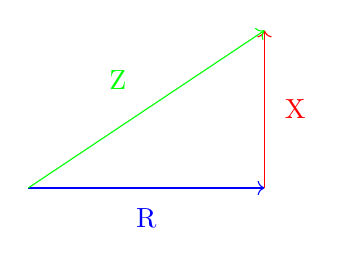
\begin{tikzpicture}
    	\draw [->,blue] (0,0) to node[label={[label distance=.01cm]-90:R}] {}(3,0);
    	\draw [->,red] (3,0) -- node[label={[label distance=.01cm]0:X}] {}(3,2);
    	\draw [->,green] (0,0) -- node[label={[label distance=.01cm]135:Z}] {}(3,2);
    	\end{tikzpicture}
    	\caption{Reactance triangle used for finding the value of the reactance.}
    \end{figure}
    
    
    Now, we can find the current on the high voltage side of the transformer using the power formula\\ $|S^H| = |I^H| \cdot |V^H|$. Rearranging we get:
    \begin{align*}
	 |I^H|	&= \frac{|S^H|}{|V^H|}\\
			&= \frac{5 \times 10^6}{66 \times 10^3}\\
			&= 75.75\si{\ampere} 
    \end{align*}
    
    Now, using a formula found in Lathi (2006), we see that:
    \begin{align*}
	    \%R^H = \frac{R^H \cdot I^H}{V^H}
    \end{align*}
    
    Rearranging, gives us:
    \begin{align*}
	    R^H &= \frac{\%R^H \cdot V^H}{I^H}\\
		    &= \frac{0.0065 \cdot 66 \times 10^3}{75.75}\\
		    &= 5.66\si{\ohm}
    \end{align*}
    
    We can find the reactance similarly:
    \begin{align*}
	    \%X^H 	&= \frac{X^H \cdot I^H}{V^H}\\
			    &= \frac{0.0898 \cdot 66 \times 10^3}{75.75}\\
			    &= 78.24\si{\ohm}	
    \end{align*}
    
    Hence, we get that the impedence on the high voltage side of the transformer is: 
    \begin{align*}
	    Z^H = (5.66 + j78.24)\si{\ohm}
    \end{align*}
    
    
    Now, since the transformers are $\Delta$-$\Delta$ connected and deliver 10$\si{\mega\watt}$ at a power factor of 0.8 (lagging) we consider the resistive power, which is given by:
    \begin{align*}
	    P_{total}^{L} 	&= 3 \cdot V_{\phi}^L \cdot I_{\phi}^L \cdot \cos(\theta)\\
					    &= 3 \cdot V_{line}^L \cdot \frac{I_{line}^L}{\sqrt{3}} \cdot \cos(\theta)\\
					    &= \sqrt{3} \cdot V_{line}^L \cdot I_{line}^L \cdot \cos(\theta)
    \end{align*}
    
    Rearranging we get an expression for $I_{line}^L$, which we solve as follows:
    \begin{align*}
	    I_{line}^L 		&= \frac{P_{total}^L}{\sqrt{3} \cdot V_{line}^L \cdot \cos(\theta)}\\
					    &= \frac{10 \times 10^ 6}{\sqrt{3} \cdot 13.2 \times 10^3 \cdot 0.8}\\
					    &= 546.73 \angle -36.86 \si{\degree} \si{\ampere}
    \end{align*}
    
    Now, we know that we can find $I_{\phi}^L$ as follows:
    \begin{align*}
	    I_{\phi}^L 	&= \frac{I_{line}^L}{\sqrt{3}}\\
				    &= 315.65 \angle -36.86 \si{\degree} \si{\ampere}
    \end{align*}
    
    Referring $I_{\phi}^L$ to the high voltage side of the transformer, we first need to work out the turns ratio:
    \begin{align*}
	    a = \frac{N_1}{N_2} = \frac{E_1}{E_2} = \frac{66}{13.2} = 5
    \end{align*}
    
    Now, we find $I_{\phi}^L$ as follows:
    \begin{align*}
	    I_{\phi}^L 	&= \frac{1}{a} \cdot I_{\phi}^H\\
				    &= \frac{1}{5} \cdot 315.65 \angle -36.86\si{\degree} \si{\ampere}\\
				    &= 63.13 \angle -36.86\si{\degree} \si{\ampere}
    \end{align*}
    
    Hence, using the equivalent circuit shown in Figure, the input voltage can be found by KVL as follows:
    \begin{align*}
	    -V_{in} + I_{\phi}^L \cdot Z^H + 66\si{\kilo\volt} = 0\\
	\end{align*}  
	
	Therefore, we get that:  
	\begin{align*}
	V_{in} 	&= I_{\phi}^L \cdot Z^H + 66\si{\kilo\volt}\\
			&= 63.13 \angle -36.86\si{\degree} \si{\ampere} \cdot (5.66 + j78.24)\si{\ohm} + 66\si{\kilo\volt}\\
			&= 69248.84 +j3737.56 \si{\kilo\volt}
    \end{align*}
    
    Hence, the input voltage is given by:\\
    \begin{center}
    	\fbox{$V_{in} = 69.35 \angle 3.08 \si{\kilo\volt}$}
    \end{center}
    
\end{homeworkProblem}
\newpage
%%%%%%%%%%%%%%%%%%%%%%%%%%%%%%%%%%%%%%%%%%%%%%%%%%%%%%%%%%%%%%%%%%%%%%%%%%%%%%%%%%%%%%%%%%%%%%%%%%%%%%%%%%%%%%%%%%%%%%
% Question 2
%%%%%%%%%%%%%%%%%%%%%%%%%%%%%%%%%%%%%%%%%%%%%%%%%%%%%%%%%%%%%%%%%%%%%%%%%%%%%%%%%%%%%%%%%%%%%%%%%%%%%%%%%%%%%%%%%%%%%%

\begin{homeworkProblem}
    
    A 9$\si{\kilo\volt\ampere}$, 208$\si{\volt}$, star connected synchronous generator has a winding resistance of 5.6$\si{\ohm\per\phi}$. Determine its voltage regulation when the power factor of the load is 80\% leading. What will is be when the power factor is 80\% leading (\textit{should this say lagging})? Show the power angle $\delta$ in a phasor diagram in both cases. Consider the full load operation.\\
    
	The equivalent circuit, for a single phase, for the synchronous generator can be seen in Figure:
    \begin{figure}[h]
    	\centering
    	\ctikzset{bipoles/length=0.8cm}
	    \begin{circuitikz}[american voltages] \draw (0,0)
		    node[draw,minimum width=2cm,minimum height=2.4cm] (load) {Load}
		    ($(load.west)!0.75!(load.north west)$) coordinate (la)
		    ($(load.west)!0.75!(load.south west)$) coordinate (lb)
		    (lb) to[short,-o] ++(-0.5,0) coordinate (b) node[below] {}
		    to[short] ++(-4,0) coordinate (VThb)
		    to[sV=$E_f$] (VThb |- la)
		    to[R=$R_a$] ++(2.5,0) coordinate (VTht)
		    to[short,-o,i=$I_L$] (VTht -| b) coordinate (a) node[above] {}
		    to[short] (la);
		    \path (a) node[below] {$+$} -- node {$V_t$} (b) node[above] {$\vphantom{+}-$};
		\end{circuitikz}
		\caption{Synchronous generator equivalent circuit}
    \end{figure}
    
    The line voltage of the synchronous generator is given in the problem statement. That is $V_{line} = 208 \angle 0 \si{\degree}$. Hence, since the synchronous generator is Y-configured, then the phase (or terminal voltage), $V_t$, is given by:
    \begin{align*}
	    V_t = \frac{V_{line}}{\sqrt{3}} = \frac{208 \angle 0\si{\degree}}{\sqrt{3}} = 120.08 \angle 0 \si{\degree} \si{\volt}
    \end{align*}
    
    Now, if the power factor is 80\% leading then, $pf = \cos(\theta) = 0.8$. If the generator is operating at full load, then we note that:
    \begin{align*}
	    P_{out} = 3 \cdot V_{\phi} \cdot I_{\phi} \cdot \cos(\theta)
    \end{align*}
    
    Rearranging, we obtain an expression for $I_{\phi}$:
    \begin{align*}
	    I_{\phi} 	&= \frac{P_{out}}{3 \cdot V_{\phi} \cdot \cos(\theta)}\\
				    &= \frac{|S_{out}| \cdot \cos(\theta)}{3 \cdot V_{\phi} \cdot \cos(\theta)}\\
				    &= \frac{9 \times 10^3}{\sqrt{3} \cdot 208}\\
				    &= 24.98 \angle 36.86\si{\degree} \si{\ampere}
    \end{align*}
    
    Now, by KVL from Figure, we see that:
    \begin{align*}
	    -E_f + I_L \cdot R_a + V_t = 0
    \end{align*}
    
    Hence, the excitation voltage, $E_f$, is given by:
    \begin{align*}
	    E_f 	&= I_L \cdot R_a + V_t\\
			    &= (24.98 \angle 36.86) \cdot 5.6 + 120.08 \angle 0 \si{\degree}\\
			    &= 139.55 \angle 36.86\si{\degree} + 120.08 \angle 0 \si{\degree}\\
			    &= 231.91 + j83.91\\
			    &= 246.62 \angle 19.89\si{\degree} \si{\volt}
    \end{align*}
    
    Now, if there is no load attached to the generator, then there is no current that flows. Hence, we get that $E_f = V_t = 120.08 \angle 0\si{\degree} \si{\volt}$.\\
    
    Finally, the voltage regulation can be calculated as:
    \begin{align*}
	    V_{reg} &= \frac{|V_{FL}| - |V_{NL}|}{|V_{NL}|}\\
			    &= \frac{246.62 - 120}{120}\\
			    &= 105.51\%
    \end{align*}
    
    \begin{center}
    	\fbox{The voltage regulation with an 80\% leading power factor for the load is 105.51\%}\\
    \end{center}
    
    If the power factor was 80\% lagging, then the phase current would be $I_{\phi} = 24.98 \angle -36.86 \si{\degree} \si{\ampere}$. Hence, when we calculate the excitation voltage, we get:
    \begin{align*}
	    E_f 	&= I_L \cdot R_a + V_t\\
	    &= (24.98 \angle -36.86) \cdot 5.6 + 120.08 \angle 0 \si{\degree}\\
	    &= 139.55 \angle -36.86\si{\degree} + 120.08 \angle 0 \si{\degree}\\
	    &= 231.91 - j83.91\\
	    &= 246.62 \angle -19.89\si{\degree} \si{\volt}
    \end{align*}
    
    Hence, we get the same voltage regulation irrespective if the 80\% power factor is leading or lagging. That is:
    
    \begin{center}
    	\fbox{The voltage regulation with an 80\% lagging power factor for the load is 105.51\%}
    \end{center}
    
    The phasor diagrams for the leading case and the lagging case can be seen in Figure and Figure, respectively.
    
     \begin{figure}[h]
     	\begin{minipage}{.5\textwidth}
     		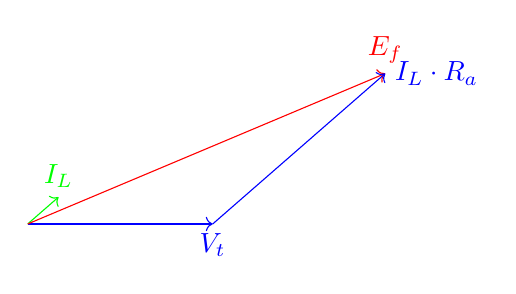
\begin{tikzpicture}
     		\begin{axis}[
     		xmin=0,
     		xmax=350,
     		ymin=-125,
     		ymax=125,
     		axis lines = none,
     		xlabel = $Re$,
     		ylabel = {$Im$}
     		]
     		
     		\addplot [blue, no markers, ->] coordinates {(0,0) (120,0)} node[below,pos=1] {$V_t$};
     		\addplot [green, no markers, ->] coordinates {(0,0) (19.98,14.98)} node[above,pos=1] {$I_L$};
     		\addplot [red, no markers, ->] coordinates {(0,0) (231.91,83.91)} node[above,pos=1] {$E_f$};
     		\addplot [blue, no markers, ->] coordinates {(120,0) (231.91,83.91)} node[right,pos=1] {$I_L \cdot R_a$};
     		
     		\end{axis}
     		\end{tikzpicture}
     		\caption{Phasor diagram for 80\% leading}
     	\end{minipage}
     	\begin{minipage}{0.5\textwidth}
     		\begin{tikzpicture}
     		\begin{axis}[
     		xmin=0,
     		xmax=350,
     		ymin=-125,
     		ymax=125,
     		axis lines = none,
     		xlabel = $Re$,
     		ylabel = {$Im$}
     		]
     		
     		\addplot [blue, no markers, ->] coordinates {(0,0) (120,0)} node[above,pos=1] {$V_t$};
     		\addplot [green, no markers, ->] coordinates {(0,0) (19.98,-14.98)} node[below,pos=1] {$I_L$};
     		\addplot [red, no markers, ->] coordinates {(0,0) (231.91,-83.91)} node[below,pos=1] {$E_f$};
     		\addplot [blue, no markers, ->] coordinates {(120,0) (231.91,-83.91)} node[right,pos=1] {$I_L \cdot R_a$};
     		
     		\end{axis}
     		\end{tikzpicture}
     		\caption{Phasor diagram for 80\% lagging}
     	\end{minipage}
     \end{figure}
     
     Finally, we the power angle $\delta$ for the leading case is given by:
     \begin{center}
     	\fbox{$\delta = 19.89\si{\degree}$}
     \end{center}
     
     The power angle $\delta$ for the lagging case is given by:
     \begin{center}
     	\fbox{$\delta = -19.89 \si{\degree}$}
     \end{center}
\end{homeworkProblem}


%%%%%%%%%%%%%%%%%%%%%%%%%%%%%%%%%%%%%%%%%%%%%%%%%%%%%%%%%%%%%%%%%%%%%%%%%%%%%%%%%%%%%%%%%%%%%%%%%%%%%%%%%%%%%%%%%%%%%%
% Question 3
%%%%%%%%%%%%%%%%%%%%%%%%%%%%%%%%%%%%%%%%%%%%%%%%%%%%%%%%%%%%%%%%%%%%%%%%%%%%%%%%%%%%%%%%%%%%%%%%%%%%%%%%%%%%%%%%%%%%%%

\begin{homeworkProblem}
    
    Three identical 500 $\si{\kilo\volt\ampere}$, 2300/230 $\si{\volt}$,single phase transformers are connected in $\delta$/Y. each transformer has Z = 0.2 + j0.6 ohms per phase equivalent impedance refereed to the HV side. The transformer bank supplies the following balanced three-phase loads at the rated low voltage:
    
    \begin{itemize}
    	\item 750 $\si{\kilo\volt\ampere}$ at 0.6 power factor lagging\\
    	\item 500 $\si{\kilo\volt\ampere}$ at 0.8 power factor lagging\\
    	\item 350 $\si{\kilo\volt\ampere}$ at unity power factor\\
    \end{itemize}
    
    Determine the primary line-to-line voltage.\\
	
	The transformers are connected to three loads and are loaded up in series as shown in Figure\\
	
	\begin{figure}[H]
		\centering
		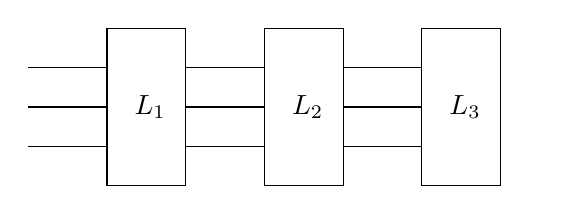
\begin{tikzpicture}
		\draw (0,0) -- (0,2) -- (1,2) -- (1,0) -- (0,0);
		\draw (2,0) -- (2,2) -- (3,2) -- (3,0) -- (2,0);
		\draw (4,0) -- (4,2) -- (5,2) -- (5,0) -- (4,0);
		\draw (-1,1) -- (0,1); \draw (1,1) -- (2,1); \draw (3,1) -- (4,1);
		\draw (-1,1.5) -- (0,1.5); \draw (1,1.5) -- (2,1.5); \draw (3,1.5) -- (4,1.5);
		\draw (-1,0.5) -- (0,0.5); \draw (1,0.5) -- (2,0.5); \draw (3,0.5) -- (4,0.5);
		
		\node[text width=1cm] at (0.85,1) {$L_1$};
		\node[text width=1cm] at (2.85,1) {$L_2$};
		\node[text width=1cm] at (4.85,1) {$L_3$};
		\end{tikzpicture}
		\caption{Three 3-$\phi$ loads connected in series.}
	\end{figure}
	
	The phase lag for load 1 is given by:
	\begin{align*}
		\theta_1 	&= \arccos(0.6)\\
					&= -53.13\si{\degree}	
	\end{align*}
	
	The phase lag for load 2 is given by:
	\begin{align*}
	\theta_2 	&= \arccos(0.8)\\
				&= -36.86\si{\degree}
	\end{align*}
	
	The phase lag for load 3 is given by:
	\begin{align*}
	\theta_3 = 0 \si{\degree}
	\end{align*}
	
	Now we can find the apparent power for each of the loads. The apparent power of the first load is given by:
	\begin{align*}
		S_1 &= 750 \angle-53.13\si{\degree} \si{\kilo\volt\ampere}\\
			&= (450 - j600) \si{\kilo\volt\ampere}
	\end{align*}
	
	The apparent power of the second load is given by:
	\begin{align*}
		S_2 &= 500 \angle -36.86 \si{\degree} \si{\kilo\volt\ampere}\\
			&= (400 - j300)\si{\kilo\volt\ampere}
	\end{align*}
	
	The apparent power of the third load is given by:
	\begin{align*}
		S_3 = 350 \angle \si{\degree} \si{\kilo\volt\ampere}
	\end{align*}
	
	The total apparent power absorbed by the loads is given by:
	\begin{align*}
		S_{total} &= S_1 + S_2 + S_3\\
			&= 450 - j600 + 400 - j300 + 350\\
			&= 1200 - j900\\
			&= 1500 \angle -36.86 \si{\degree} \si{\kilo\volt\ampere}
	\end{align*}
	
	Now, we can find the phase current, $I_{\phi}^L$, using the following relationship:
	\begin{align*}
		|S_{total}^L| = 3 \cdot |S_{\phi}^L| = 3 \cdot |V_{\phi}^L| \cdot |I_{\phi}^L|
	\end{align*}
	
	rearranging, we get that:
	\begin{align*}
		|I_{\phi}^L| 	&= \frac{|S_{total}|}{3 \cdot |V_{\phi}|}\\
						&= \frac{1500 \times 10^3}{3 \cdot 230}\\
						&= 2173.91 \si{\ampere}
	\end{align*}
	
	Hence, the current is given by:
	\begin{align*}
		I_{\phi}^L = 2173.91  \angle -36.86 \si{\degree} \si{\ampere}
	\end{align*}
	
	Now, we can refer the current, $I_{\phi}^L$, to the high voltage side, using the turns ratio. The turns ratio is given by:
	\begin{align*}
		a = \frac{N_1}{N_2} = \frac{E_1}{E_2} = \frac{2300}{230} = 10
	\end{align*}
	
	Hence, we find $I_{\phi}^H$, as follows:
	\begin{align*}
		I_{\phi}^H 	&= \frac{1}{a} \cdot I_{\phi}^L\\
					&= \frac{1}{10} \cdot 2173.91 \angle -36.86\si{\degree}\\
					&= 217.39 \angle -36.86 \si{\degree} \si{\ampere}	
	\end{align*}
	
	Finally, we can find the line to line voltage (which is the same as the phase voltage for a $\Delta$-circuit) using a KVL on the equivalent circuit shown in Figure:
	\begin{align*}
		-V_{line}^H + I_{line}^H \cdot Z_{line}^H + 2300 = 0\\
	\end{align*}
	
	Therefore, we get that:
	\begin{align*}
		V_{line}^H 	&= I_{line}^H \cdot Z_{line}^H + 2300 \angle 0\si{\degree}\\
					&= 217.39 \angle -36.86 \si{\degree} \si{\ampere} \cdot (0.2 + j0.6) +2300 \angle 0 \si{\degree}\\
					&= 137.39 \angle 34.70 \si{\degree} + 2300 \angle 0 \si{\degree}\\
					&= 112.88 + j78.16 + 2300\\
					&= 2412.88 + j78.16
	\end{align*}
	
	Hence the line to line voltage of the transformer is given by:
	\begin{center}
		\fbox{$V_{line}^H = 2414.15 \angle 1.85 \si{\degree} \si{\volt}$}
	\end{center}
	
\end{homeworkProblem}

%%%%%%%%%%%%%%%%%%%%%%%%%%%%%%%%%%%%%%%%%%%%%%%%%%%%%%%%%%%%%%%%%%%%%%%%%%%%%%%%%%%%%%%%%%%%%%%%%%%%%%%%%%%%%%%%%%%%%%
% Question 4
%%%%%%%%%%%%%%%%%%%%%%%%%%%%%%%%%%%%%%%%%%%%%%%%%%%%%%%%%%%%%%%%%%%%%%%%%%%%%%%%%%%%%%%%%%%%%%%%%%%%%%%%%%%%%%%%%%%%%%

\begin{homeworkProblem}
    A 6-pole, 230$\si{\volt}$, 60$\si{\hertz}$, star connected, three phase induction motor has the following parameters on a per phase basis:
    \begin{multicols}{2}
    \begin{itemize}
    	\item $R_1 = 0.5\si{\ohm}$
    	\item $R_2 = 0.25\si{\ohm}$
    	\item $X_1 = 0.75\si{\ohm}$
    	\item $X_2 = 0.5\si{\ohm}$
    	\item $X_m = 100\si{\ohm}$
    	\item $R_c = 500\si{\ohm}$
    \end{itemize}
	\end{multicols}
	
	All the impedances are refereed to the stator side. The friction and windage loss is 150 watts. Determine the efficeincy of the motor at its rated slip of 2.5\%.\\
	
	The motor is Y-connected, so given that $V_{line} = 230\si{\volt}$, then:
	\begin{align*}
		V_{\phi} = \frac{V_{line}}{\sqrt{3}} = \frac{230 \angle 0 \si{\degree}}{\sqrt{3}} = 132.79 \angle 0\si{\degree} \si{\volt}
	\end{align*}
	
	The equivalent circuit for the induction motor, which includes both $R_C$ and $X_m$, is shown in Figure:
	\begin{figure}[h]
		\centering
		\ctikzset{bipoles/length=0.8cm}
		\begin{circuitikz}
			\draw
			(0,2) 
			to [short,i=$I_1$,o-](2,2)
			to[R,l=$R_1$] (4,2)
			to[L,l=$X_1$,i=$I'_2$] (6,2) 
			to[L, l=$X'_2$] (8,2)
			to[R, l=$\frac{R'_2}{s}$] (8,0)
			to[short,-o] (0,0)
			;
			\draw
			(1.5,2) to [short,i=$I_{\phi}$](1.5,1.5) -- (1,1.5)
			to[R,l_=$R_C$](1,0);
			\draw
			(1.5,1.5) -- (2,1.5)
			to[L,l=$X_m$](2,0)
			;
			\draw (0,1) to [short,l=$V_1$](0,1);
		\end{circuitikz}
		\caption{Equivalent circuit for the induction motor described in the problem.}
	\end{figure}
	
	Therefore, with reference to Figure, we see that:
	\begin{align*}
		I'_2 	&= \frac{V_1}{Z^eq}\\
				&= \frac{V_1}{R_1 + jX_1 + jX'_2 + \frac{R'_2}{s}}\\
				&= \frac{132.79 \angle 0\si{\degree}}{0.5 + \frac{0.25}{0.025} + j(0.75 + 0.5)}\\
				&= \frac{132.79 \angle 0 \si{\degree}}{10.57 \angle 6.79 \si{\degree}}\\
				&= 12.56 \angle -6.79 \si{\degree} \si{\ampere}
	\end{align*}
	
	Further, we can find the current, $I_{\phi}$, in the excitation branch using:
	\begin{align*}
		I_{\phi} = \frac{V_1}{Z_{\phi}^{eq}}
	\end{align*}
	
	We have $R_C$ and $X_m$ are in parallel, hence, we can find that:
	\begin{align*}
		Z_{\phi}^{eq} = \bigg(\frac{1}{R_C} + \frac{1}{jX_m}\bigg)^{-1} = 98.06 \angle 78.69 \si{\degree}
	\end{align*}
	
	Hence, the current in the excitation branch is given by:
	\begin{align*}
		I_{\phi} = \frac{V_1}{Z_{\phi}^{eq}} = \frac{132.79 \angle 0 \si{\degree}}{98.06 \angle 78.69 \si{\degree}} = 1.35 \angle -78.69 \si{\degree} \si{\ampere}
	\end{align*}
	
	Finally, we can find the current $I_1$ as follows:
	\begin{align*}
		I_1 &= I_{\phi} + I_{2}\\
			&= 1.35 \angle -78.69 \si{\degree} + 12.56 \angle -6.79\\
			&= 0.2647 -j1.323 + 12.47 - j1.4849\\
			&= 12.73 - j2.80\\
			&= 13.03 \angle -12.40 \si{\degree} \si{\ampere}
	\end{align*}
	
	Now, we can find the apparent input power as follows:
	\begin{align*}
		S_{in} 	&= 3 \cdot V_1 \cdot I_1^*\\
				&= 3 \cdot 132.79 \angle 0 \si{\degree} \cdot 13.03 \angle 12.40 \si{\degree}\\
				&= 5190.76 \angle 12.40 \si{\degree} \si{\volt\ampere}
	\end{align*}
	
	Hence the input power is given by:
	\begin{align*}
		P_{in} = 5190.76 \cos(12.40 \si{\degree}) = 5069.67 \si{\watt}
	\end{align*}
	
	Now, the air gap power, $P_{ag}$, is given by the formula:
	\begin{align*}
		P_{ag} 	&= 3 \cdot I_2^2 \cdot \frac{R_2}{s}\\
				&= 3 \cdot (12.56)^2 \cdot \frac{0.25}{0.025}\\
				&= 4732.61 \si{\watt}
	\end{align*}
	
	Then we can find the mechanical power, $P_{mech}$, as follows:
	\begin{align*}
		P_{mech} 	&= P_{ag} \cdot (1 - s)\\
					&= 4732.61 \cdot (1 - 0.025)\\
					&= 4614.29 \si{\watt}
	\end{align*}
	
	Finally, we find that the output power, $P_{out}$, is given by:
	\begin{align*}
		P_{out} = P_{mech} - P_{f+w} = 4614.29 - 150 = 4464.29 \si{\watt}
	\end{align*}
	
	Finally, the effienicy is given by:
	\begin{center}
		\fbox{$\eta = \frac{P_{out}}{P_{in}} = \frac{4464.29}{5069.67} = 88.05\%$}
	\end{center}
	
\end{homeworkProblem}

	
	
	
\end{document}
